% -%-%-%-%-%-%-%-%-%-%-%-%-%-%-%
% INFMDI 348  
% Date:09/06/2012 
% Paris,France  
% Groupe: 
% - Tiago CHEDRAOUI SILVA 
% - Livia RIBEIRO 
% - Anthony CLERBOUT
% -%-%-%-%-%-%-%-%-%-%-%-%-%-%-%

\documentclass[a4paper,11pt]{article}

\usepackage[english,listings,algo]{tcs}

% Cover %
\def \ttprofname{Mauro Sozio} % teachers name
\def \ttabrv{INFMDI348} % abbreviation of names class
\def \ttabrvxt{} % period
\def \mytitle{Project on Data Mining} % Big title
\def \mysubtitle{Clustering} % subtitle
\def \ttauthi{Tiago CHEDRAUOI SILVA} % author's name
\def \ttdate{June 22, 2012} % date

\begin{document}
\titleTMB 
\newpage
\tableofcontents
\listoffigures
\newpage

\section{Introduction}
The main goal of this project is to clustering a collection of documents so that documents dealing with a same topic belong to a same cluster.
To this purpose, we chose to use the k-means algorithm.

\section{Pre-processing}
 As  input for  the  clustering we  have  1000 documents  that  were taken  from
 blogs. Some steps to remove noisy are applied: 
1. Remove non-alphabetic characters
2. Remove white spaces
3. Make every word lower case
4. Remove stopwords
5. Remove  Words with  frequency lower than  5 times  and higher than  1000 (ex:
object, message, from, etc.), because  they are considered noises as they cannot
give a meaningful value to our clustering.
6. Normalize the matrix: That  gives the same importance
to all documents: either a big or  a small document will have the same influence
during a cluterization.


%\begin{enumerate}
%\item Remove non-alphabetic characters
%\item Remove white spaces
%\item Make every word lower case
%\item Remove stopwords
%\item Remove Words with extremely low or high frequency
%\item Normalize the matrix
%\end{enumerate}

After the step 5 on the pre-processing, we make a histogram of the words, which shows that the
major part of words have a low frequency, and some words have a high frequency.
The important words are those which appears in a great part of
documents with high frequency, which could induce us to a cluster.
For  example, if  my files  talk about  sports and  are recent  maybe  the word
Eurocup and  Olympic games have  a high frequency  and appears in most  part of
documents with sports subject. 

\begin{figure}[h!]
  \begin{centering}
    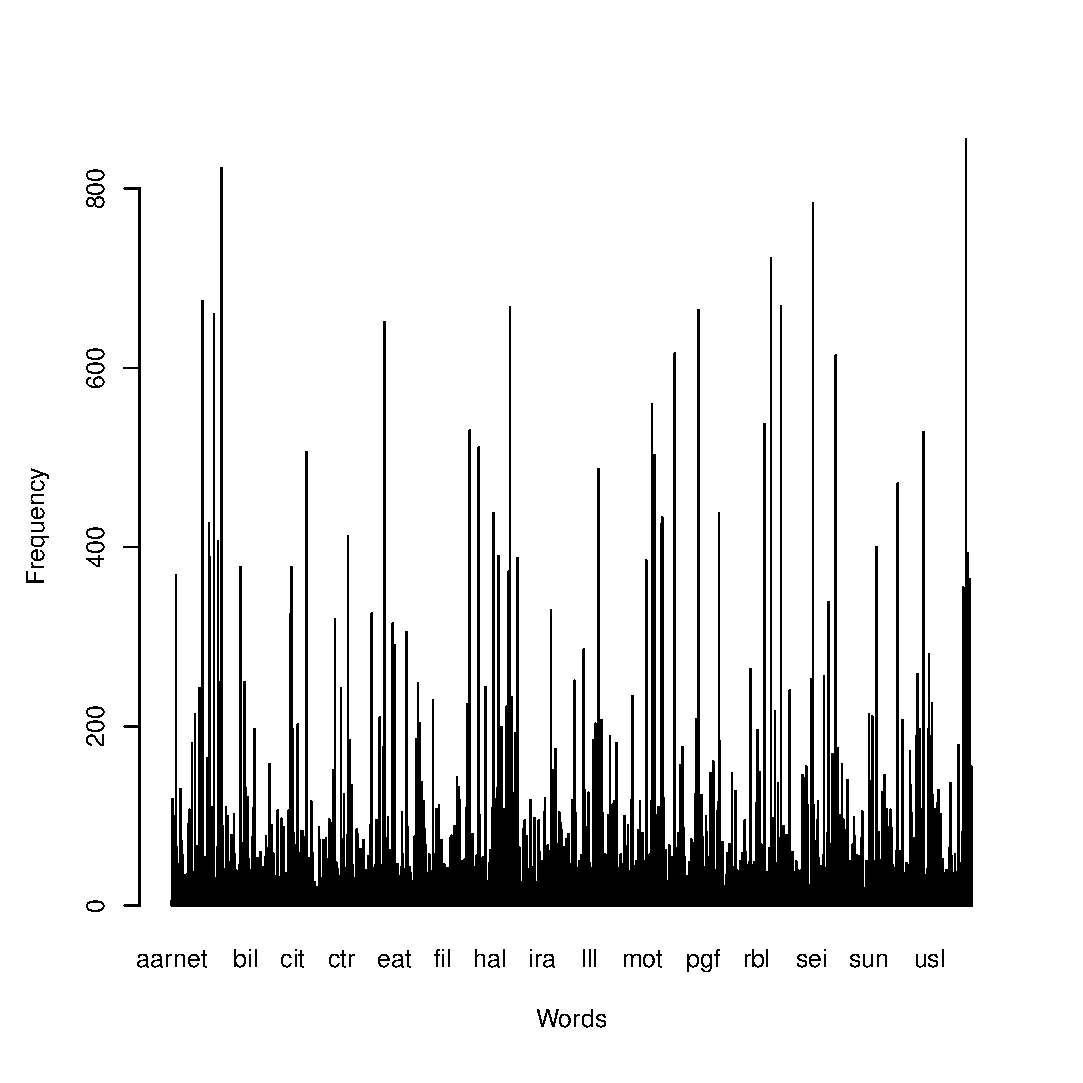
\includegraphics[trim=0 0 0 50,scale=0.5]{../graphs/q1/Histogram}
    \par\end{centering}
  \caption{Histogram word frequency in a collection of documents}
  \label{fig:jacobi-conv}
\end{figure}



\section{Clustering}

%\begin{multicols}{2}
%  \lstinputlisting[title=\textbf{Kmeans:Example of empty cluster}]{../kmeans.R}
%\end{multicols}

%Q3
An algorithm  that clusters  a given points  is the k-means  algorithm, which
needs as input  a number of clusters and  the data. The steps are:  find to each
point the  nearest center,  so that my  point belongs  to the cluster  with that
center.  After  we  recalculate  the   centers  and  restart.  We  stop  if  the
recalculates centers are unchanged.

So, we executed k-means (k = 3) on our corpus 10 times, each one with different initial centers. The best result is showed in table \ref{tab:kmens3}:
\begin{table}[H]
  \caption{Clustering Results}
  \label{tab:kmens3}

  \begin{center}
    \begin{tabular}{|l|l|}
      \hline
      \multicolumn{2}{|c|}{K-means (k = 3)}\\
      \hline
      \hline
      Size Group 1& 389 \\
      Size Group 2& 224 \\
      Size Group 3& 508\\
      \hline
      SSE & 999.9103 \\
      \hline
    \end{tabular}
  \end{center}
\end{table}

Unfortunately, the k-means algorithm can produce an empty cluster.
To show an example  of empty cluster, we have chosen some  points and centers so
that in an iteration,  a recalculated center is more far from  one point in its
cluster than the center of another cluster. 
If all points of a cluster are closer to other cluster centers, then the next iteration the cluster will be emptied.

The figure \ref{fig:emptya} shows the initial points and centers. After the 
first interaction, we have 3 cluster (blue: 1 point, black: 2 point, red: 4
point) showed in the figure \ref{fig:emptyb}. Finally the figure \ref{fig:emptyc}
shows that after the recalculation of the
centers, we got an empty cluster (blue: 2 point, black: empty, red: 5 points)

\begin{figure}[ht!]
  \begin{centering}
    \subfigure[Initial Points]{
      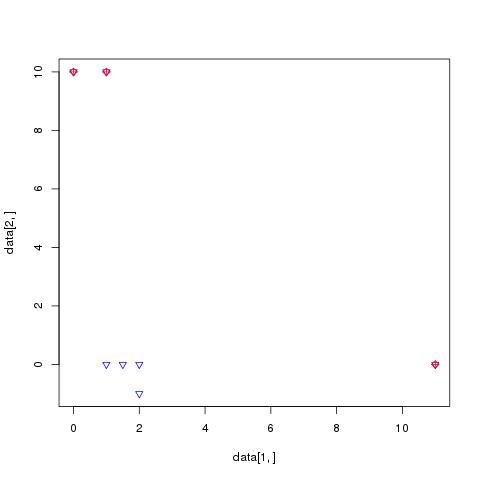
\includegraphics[trim = 0 0 50 50,scale=0.35]{../graphs/q2/InitialPoints}
      \label{fig:emptya}
    }
    \subfigure[Iteration 1]{
      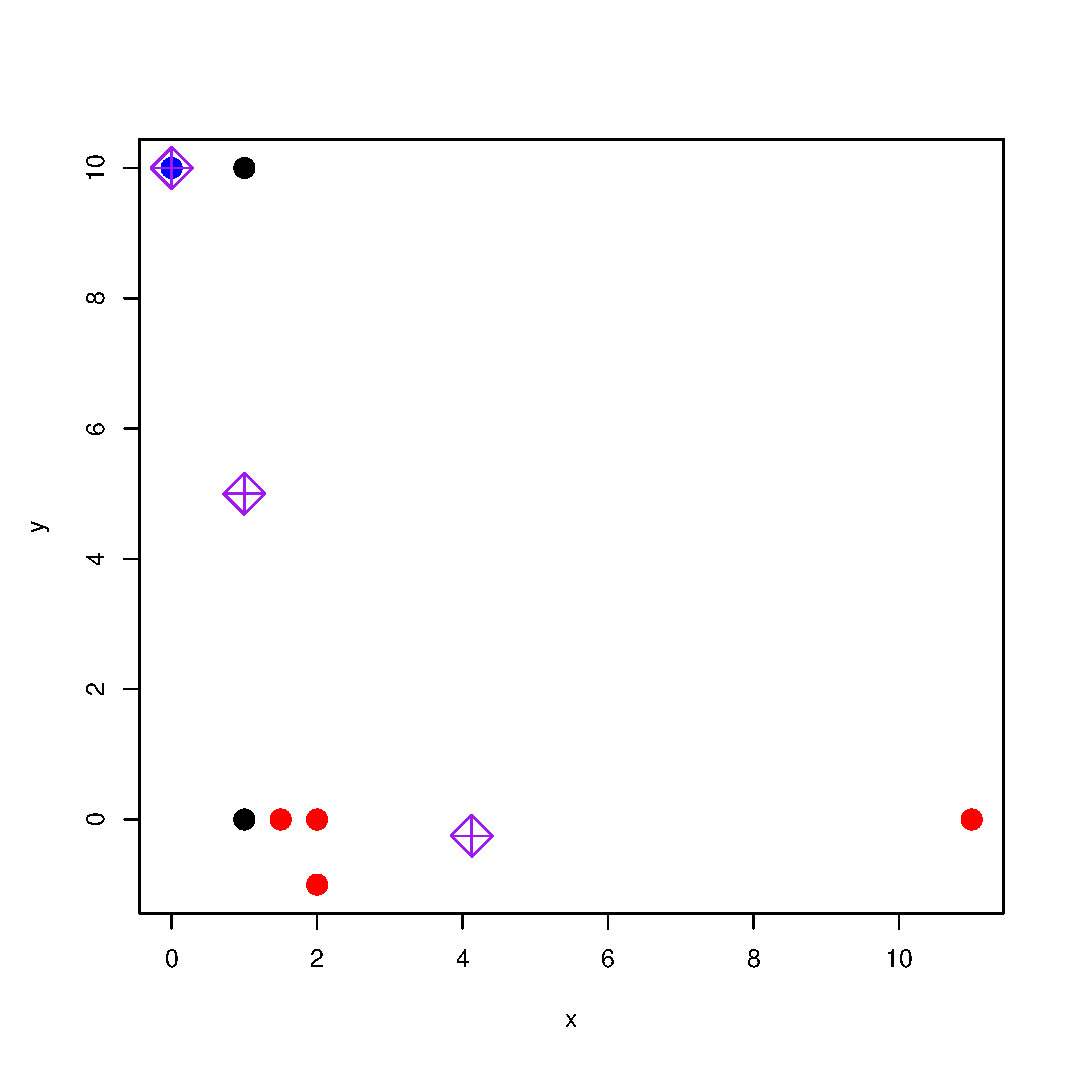
\includegraphics[trim = 0 0 50 50,scale=0.35]{../graphs/q2/0Empty}
      \label{fig:emptyb}
    }
    \subfigure[Iteration 2]{
      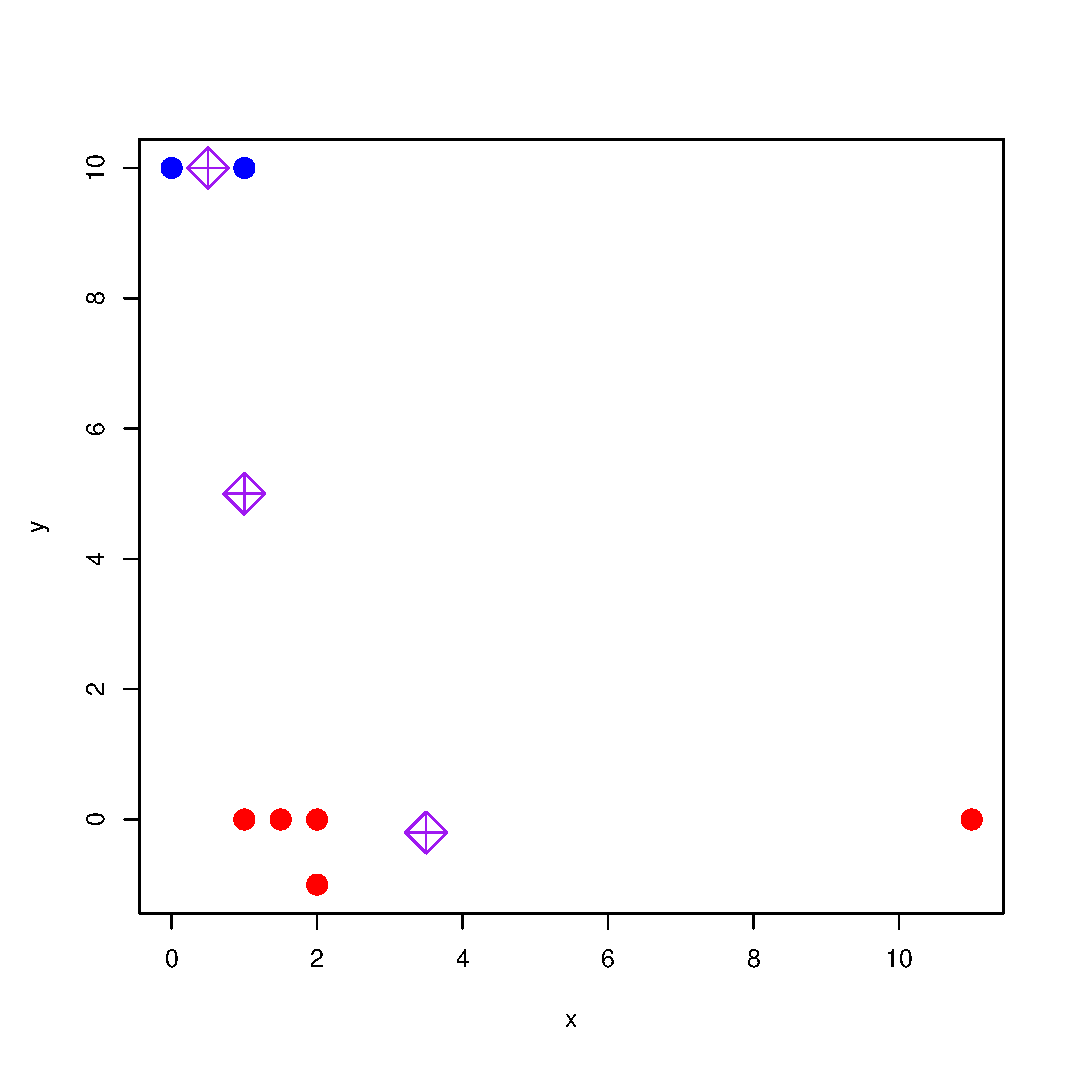
\includegraphics[trim=0 0 50 50,scale=0.35]{../graphs/q2/1Empty}
      \label{fig:emptyc}
    }
  \end{centering}
  \caption{Kmeans: Example of empty cluster}
  \label{fig:empty}

\end{figure}
  
% http://www.stanford.edu/~hastie/Papers/gap.pdf
\subsection{Clustering validation}

A  great number  of  studies were  made to  validate  a clustering  such as  Gap
statistics, silhouette validation technique and the Hartigan calculus. These algorithms give us the best
number of cluster to the data based on the solution for different number of clusters.

 The  average silhouette  width could  be applied  for evaluation  of clustering
 validity and also  could be used to  decide how good is the  number of selected
 clusters. To construct the silhouettes S(i) the following formula is used:

\begin{equation}
S_i = \frac{b_i-a_i}{max(a_i,b_i)}
\end{equation}

Where $a_i$ is  average distance of the  sample to all other samples  in the same
cluster and  $b_i$ is the  lowest average distance to the other
clusters, that means, we get all points from other clusters and we make get the
average distance to our sample point. As each different cluster give us a value,
we get the lowest one.

So the idea is to maximize the distance between different clusters and minimize the distance
of the points in the same cluster.

As a result we get a $-1 < s_i < 1$, if $s_i$ is near 1 we have a well clustered
point, if it is near -1 we have as misclassification, if it is near 0 the sample
could be assigned to other cluster. We search for the maximum value o the average
$s_i$ which means  that the points were more near to  a well clustering than
lower values.

So, using the method of average silhouette coefficient which combines both 
cohesion and separation we got the graph \ref{fig:kb}, which gives $k_{good} = 4$.


%The first simple analysis is the calculus of SSE (sum of the squared error
%)for differents values of k.
%It  is  obvious  that increasing  k  lead  us  to  a  small value  of  SSE  (see
%figure \label{fig:kSSE}). So we need to choose the k where we have an elbow. In
%figure \label{fig:kSSE} this knee is found in  $k_{good} = 5$

%Hartigan (1975) proposed the statistic:
Also Hartigan in 1975 used the SSE value as a value for comparison. Firstly, as
the SSE value always  decrease with the increase of k, Hartigan  tried to give a
penalty value for increasing the k, also he would compared the value of SSE of k
and k+1, which give us the Hartigan's method equation:

\begin{equation*}
H(k) = \left ( \frac{W(k)}{W(k+1)}-1  \right )*(n-k-1)
\end{equation*}

where  n is  the number  of instances  being clustered  and k  is the  number of
sets. Hartigan suggests that if H(k) > 10 the cluster should be added, if H(k)<10,
the cluster  is not added and the  algorithm is stop. Applying  Hartigan, we got
the graph \ref{fig:ka} which gives $k_{good} = 4$

Finally, as both methods, which are a reference in the field of study, gave us $k_{good} = 4$, we will use this value for the next experiments. 
However, that doesn't mean that it is the real best number of clusters.

\begin{figure}[ht!]
  \begin{centering}
    \subfigure[SSE vs k]{
    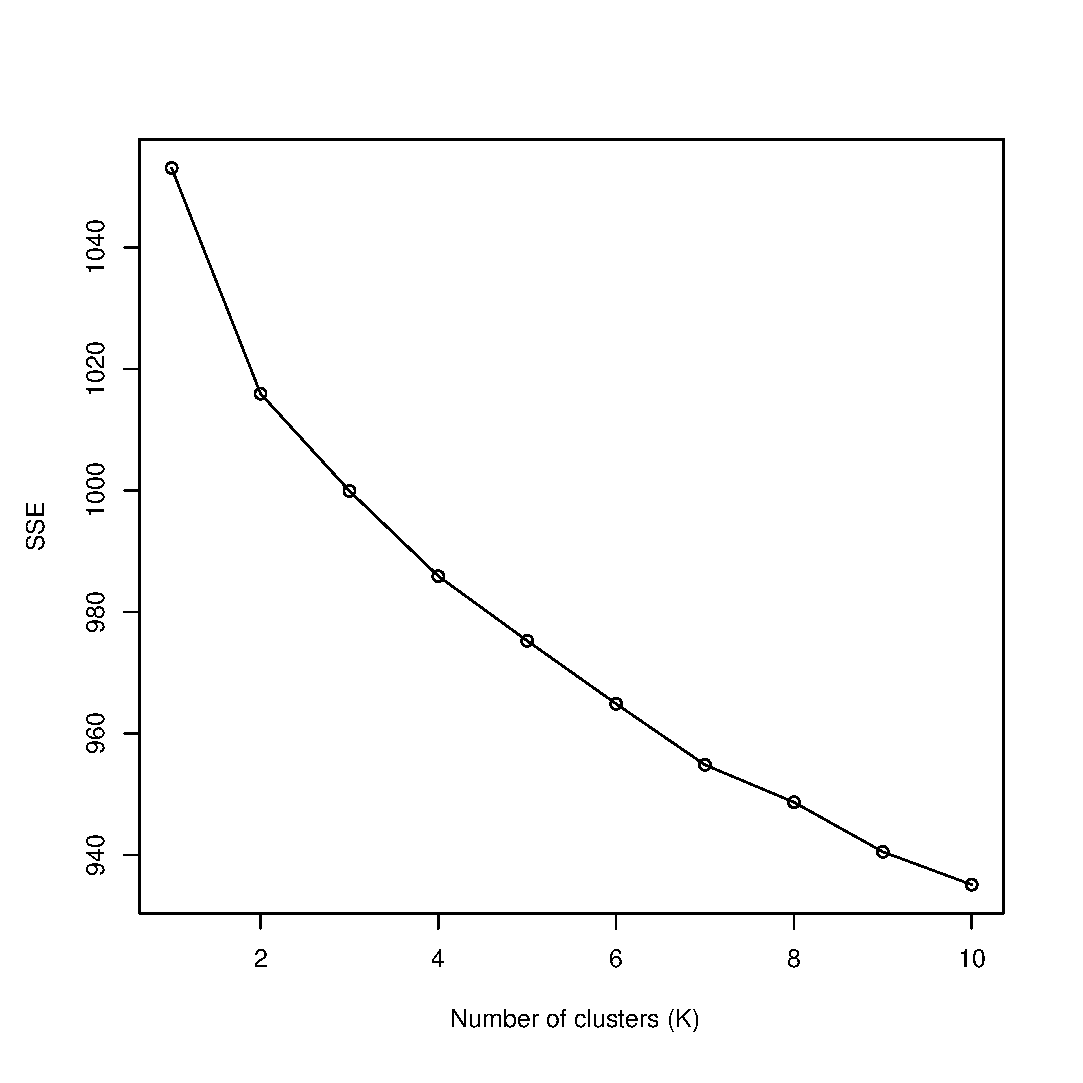
\includegraphics[trim=0 0 50 50, scale = 0.35]{../graphs/q4/SSEerror}
      \label{fig:kSSE}
    }
   \subfigure[Hartigan Calculus]{
      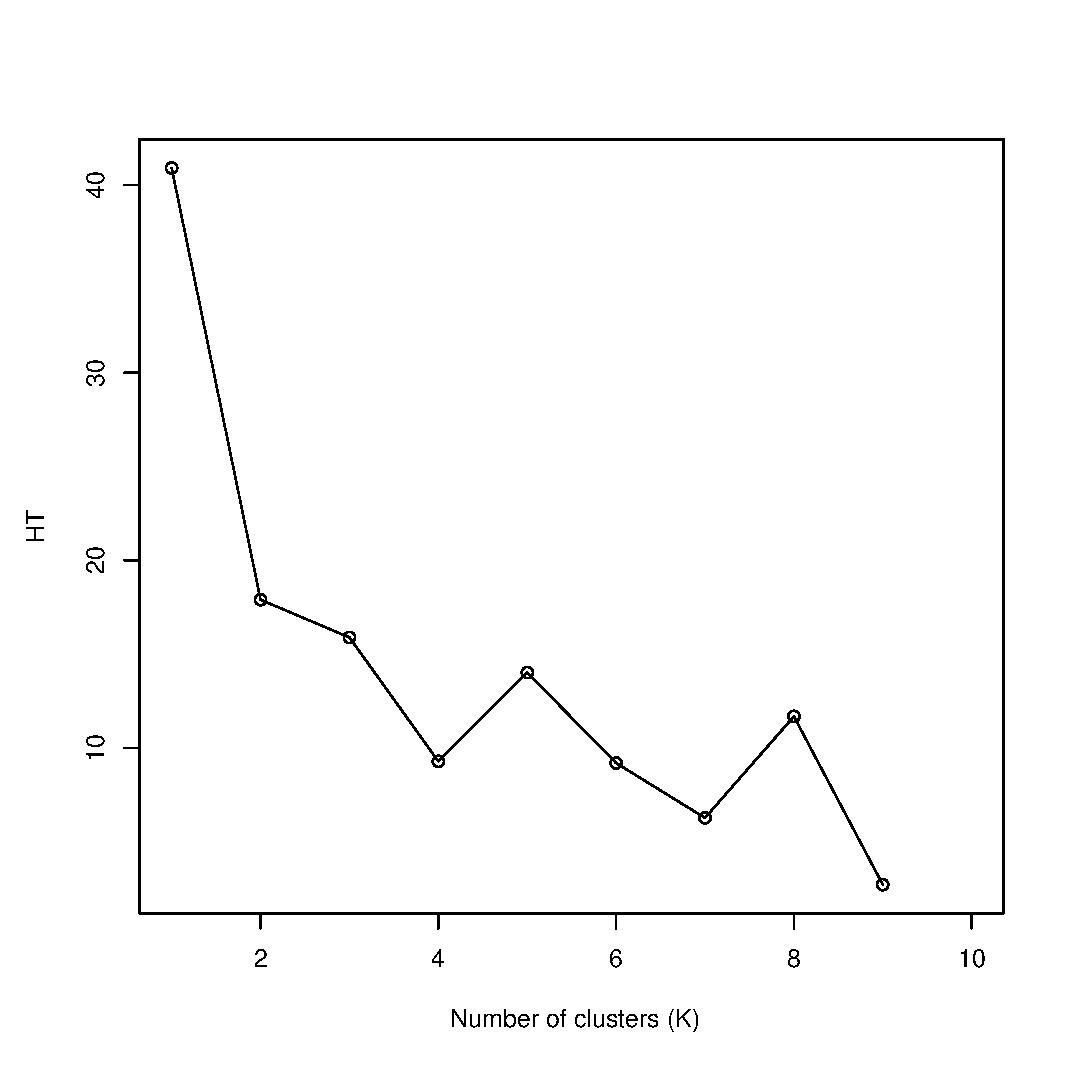
\includegraphics[trim = 0 0 50 50, scale = 0.35]{../graphs/q4/HT}
      \label{fig:ka}
    }
    \subfigure[Silhouette  Coefficient]{
      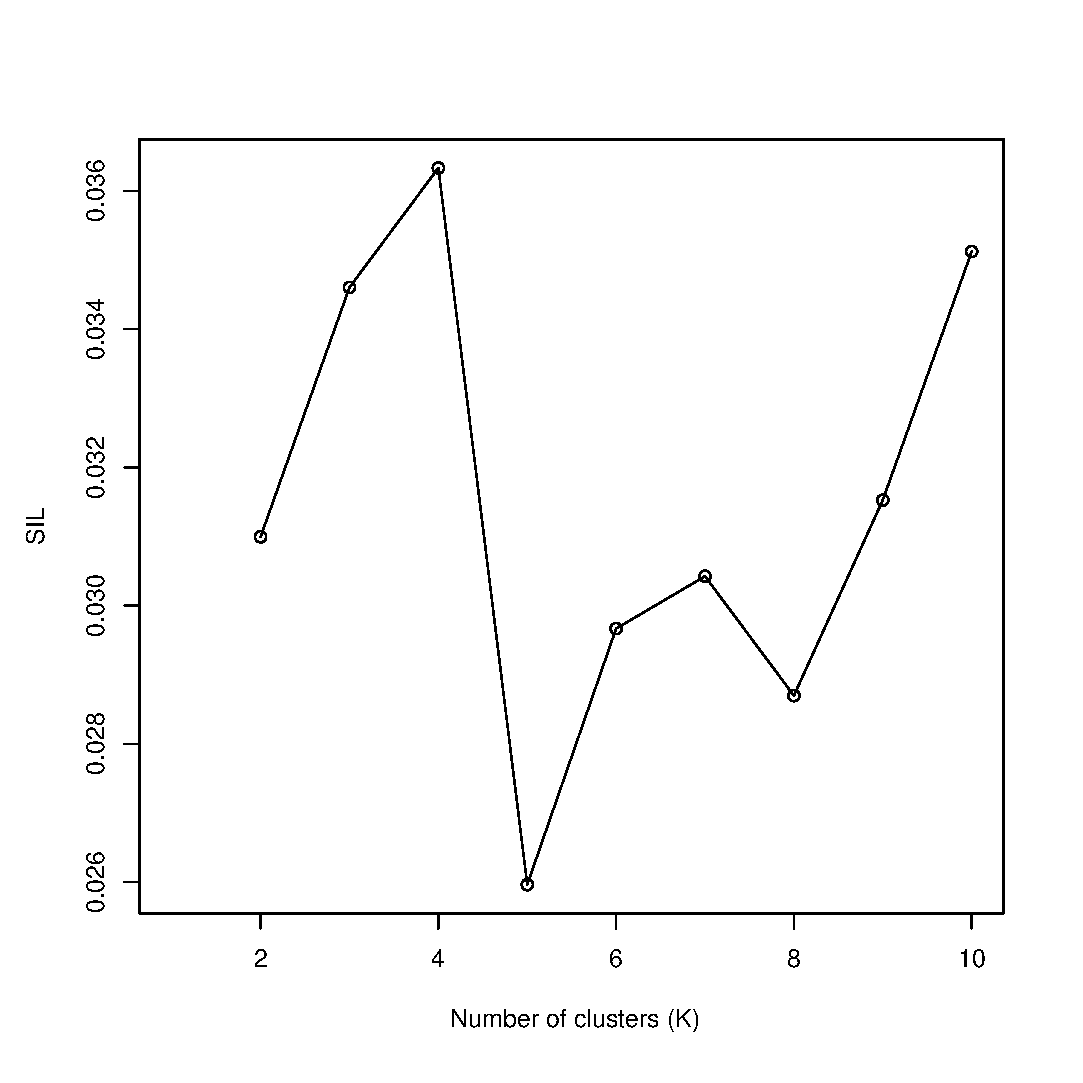
\includegraphics[trim = 0 0 50 50, scale = 0.35]{../graphs/q4/SIL}
      \label{fig:kb}
    }
  \end{centering}
  \caption{Kmeans validation}
  \label{fig:val}
\end{figure}

\subsection{Clustering Analyses}

For the  analyses of a clustering  we fixed $k  = 4$ and developed  the functions
that calculates the purity and entropy of each cluster. As k is fixed, the 
parameter that  have a great influence  in the k-means algorithm  is the initial
centers. The table below shows the result when the centers are fixed and when we
increase the times  of the random starts. This shows that  greater is the number
of starts the probability of a better result is increased. Also, a 


\begin{table}[ht!]
  \caption{Results k-means }
  \begin{centering}
    \begin{tabular}{|c|c|c|c|c|c|c|c|c|c|c|c|c|c|c|}
      \cline{2-15} 
      \multicolumn{1}{c|}{} & Time & SSE & \multicolumn{4}{c|}{Distrib} & \multicolumn{4}{c|}{Purity} & \multicolumn{4}{c|}{Entropy}\tabularnewline
      \hline 
      Fixed & 0.028 & 987.42 & 367 & 381 & 218 & 155 & 0.59 & 1 & 0.94 & 0.98 & 1.34 & 0 & -0.30 & -0.99\tabularnewline
      \hline 
      Rand (nstart = 1) & 0.044 & 988.28 & 301 & 222 & 434 & 164 & 0.98 & 1 & 0.74 & 1 & 0.11 & 0 & 1.08 & 0\tabularnewline
      \hline 
      Rand (nstart = 5) & 0.273 & 986.35 & 383 & 219 & 422 & 97 & 1 & 0.94 & 0.65 & 0.98 & 0 & 0.30 & 1.23 & 0.08\tabularnewline
      \hline 
      Rand (nstart = 10) & 0.323 & 986.35 & 383 & 97 & 422 & 219 & 1 & 0.99 & 0.65 & 0.94 & 0 & 0.08 & 1.23 & 0.30\tabularnewline
      \hline 
      Rand (nstart = 20) & 0.57 & 985.88 & 77 & 384 & 219 & 441 & 0.99 & 1 & 0.94 & 0.66 & 0.1 & 0 & 0.3 & 1.2\tabularnewline
      \hline 
    \end{tabular}
    \par\end{centering}
  
  
\end{table}

\section{References}
Hartigan, J. (1975) Clustering Algorithms New York: Wiley

http://www.stanford.edu/~hastie/Papers/gap.pdf

\end{document}

